\chapter{Zásuvný modul}
\label{plugin}

V~této kapitole je popsán samotný zásuvný modul. Pro~názornost
a~srozumitelnost jsou zde uvedeny důležité části kódu a~diagramy
znázorňující složitější algoritmy.

Kapitola se věnuje zejména technickému řešení a~jeho důvodům. Popis
toho, k~čemu jednotlivé prvky grafického uživatelského rozhraní
slouží, je obsahem uživatelského manuálu, viz
příloha~\ref{uzivatelsky_manual}.

	\begin{figure}[H] \centering
		
\includegraphics[width=.1\textwidth]{./pictures/puplugin.png}
		\caption[Zásuvný modul~– ikona]{Zásuvný modul~– ikona (zdroj: autor)}
		\label{fig:ikona_pluginu}
 	\end{figure}

\section{Vývoj}
\label{vyvoj}

Vývoj projektu probíhal pomocí verzovacího systému
Git, zdrojový kód je dostupný
v~GitHub repositáři\footnote{\url{https://github.com/ctu-geoforall-lab-projects/dp-svoboda-2017}}.

Pro~vytvoření základní kostry pluginu byl použit zásuvný modul
\textit{Plugin Builder}, který je součástí oficiálního repositáře
programu QGIS\footnote{\label{oficialni_repositar_qgis}\url{http://plugins.qgis.org/}}. Postupem času
byly ovšem názvy tříd, modulů a~celá struktura zásuvného modulu
změněny.

K~testování a~ladění byly použity další zásuvné moduly \textit{Remote
Debug}, \textit{Plugin Reloader} a~\textit{ScriptRunner}, jež jsou rovněž
dostupné z oficiálního repositáře\footnoteref{oficialni_repositar_qgis}.

Během~vývoje zásuvného modulu bylo čerpáno z~literatury zabývající se
programem QGIS \citep{pyqgis_book}, programovacím jazykem Python
\citep{python3_oop_book}~\citep{dive_into_python} a~modulem PyQt
\citep{pyqt_book}.

\section{Grafické uživatelské rozhraní}
\label{gui}

Grafické uživatelské rozhraní zásuvného modulu je reprezentováno
jedním oknem třídy
\texttt{QDockWidget}\footnote{\url{http://pyqt.sourceforge.net/Docs/PyQt4/qdockwidget.html}},
jehož hlavní výhodou je možnost ukotvení do~samotného programu
QGIS. Díky tomu není nutné přepínat mezi~okny a~práce s~pluginem se
stává uživatelsky přívětivou.

Protože zásuvný modul se řídí podle~legislativy České republiky
a~používá výmě\-nný formát katastru nemovitostí, je grafické
uživatelské rozhraní v~českém jazyce.

\section{Načtení VFK souboru}
\label{nacteni_vfk}

Soubor \zk{VFK} obsahuje mnoho datových bloků, pro~pozemkové úpravy je
tím nej\-důležitějším vrstva parcel (\texttt{\zk{PAR}}).

\subsection{Algoritmus}
\label{nacteni_vfk_algoritmus}

Algoritmus pro načtení vrstvy parcel ze~souboru \zk{VFK} patří mezi
komplikovanější části zásuvného modulu a~je klíčový pro~správný chod
navazujících procesů.

První verze tohoto algoritmu byla inspirována \zk{VFK}
Pluginem\footnote{\url{\detokenize{https://github.com/ctu-geoforall-lab/qgis-vfk-plugin}}},
ale během vývoje bylo nezbytné algoritmus mnohokrát upravovat
a~ve~výsledku se dosti liší.

Pro čtení \zk{VFK} souborů používá QGIS knihovnu GDAL (viz kapitola
č.~\ref{podklady}), konkrétně se jedná o \zk{VFK}
Driver\footnote{\url{\detokenize{http://www.gdal.org/drv_vfk.html}}}. Ten
funguje tak, že při prvním čtení souboru vytvoří ve stejném adresáři,
ve kterém se nachází čtený \zk{VFK} soubor, SQLite databázi a~do~ní
naimportuje všechna data. Při~dalším čtení se již databáze nevytváří,
proto je čtení mnohonásobně rychlejší, viz
tab.~\ref{tab:nacteni_vfk_driver}.

%%% ML: uvest testovaci soubor (asi ten ze strane CUZK, je to tak?)
\begin{table}[H]
    \begin{tabular}{|l|l|} \hline načtení & čas [s] \\ \hline \hline
první & 6.516 \\ \hline opakované & 0.160 \\ \hline
    \end{tabular} \centering
    \caption[VFK Driverem~– porovnání rychlosti načtení]{VFK
Driverem~– porovnání rychlosti načtení (zdroj: autor)}
    \label{tab:nacteni_vfk_driver}
\end{table}

\zk{VFK} Driver ovšem umožňuje otevřít \zk{VFK} soubor pouze v~režimu
čtení a~to je pro~potřeby zpracování pozemkových úprav nedostatečné.

Pro~takové případy je knihovna GDAL vybavena SQLite
Driverem\footnote{\url{\detokenize{http://gdal.org/drv_sqlite.html}}},
který nabízí možnost zápisu do SQLite databáze. Aby byl SQLite driver
schopen rozpoznat a~přečíst geometrii, musí databáze obsahovat tabulky
\texttt{\detokenize{geometry_columns}}
a~\texttt{\detokenize{spatial-}}\\\texttt{\detokenize{_ref_sys}}. V~tabulce
\texttt{\detokenize{geometry_columns}} je uveden seznam tabulek, které
mají geo\-metrii, společně s~údaji jako název sloupce s~geometrií, typ
geometrie, souřadnicový systém a~další, viz
tab.~\ref{tab:geometry_columns}. Údaje o~souřadnicovém systému
odkazují na~tabulku \texttt{\detokenize{spatial_ref_sys}}, ve~které
jsou souřadnicové systémy definovány. Seznam sloupců tabulky
\texttt{\detokenize{spatial_ref_sys}} a~jejich datové typy popisuje
tab.~\ref{tab:spatial_ref_sys}.

\begin{table}[H]
    \begin{tabular}{|l|l|} \hline název sloupce & datový typ \\ \hline
\hline \texttt{\detokenize{F_TABLE_NAME}} & \texttt{varchar unique} \\
\hline \texttt{\detokenize{F_GEOMETRY_COLUMN}} & \texttt{varchar} \\
\hline \texttt{\detokenize{GEOMETRY_TYPE}} & \texttt{integer} \\
\hline \texttt{\detokenize{COORD_DIMENSION}} & \texttt{integer} \\
\hline \texttt{\detokenize{SRID}} & \texttt{integer} \\ \hline
\texttt{\detokenize{GEOMETRY_FORMAT}} & \texttt{varchar} \\ \hline
    \end{tabular} \centering
    \caption[Tabulka \texttt{geometry\textunderscore columns}~–
sloupce]{Tabulka \texttt{geometry\textunderscore columns}~– sloupce (zdroj: autor)}
    \label{tab:geometry_columns}
\end{table}

\begin{table}[H]
    \begin{tabular}{|l|l|} \hline název sloupce & datový typ \\ \hline
\hline \texttt{\detokenize{SRID}} & \texttt{integer unique} \\ \hline
\texttt{\detokenize{AUTH_NAME}} & \texttt{text} \\ \hline
\texttt{\detokenize{AUTH_SRID}} & \texttt{tex}t \\ \hline
\texttt{\detokenize{SRTEXT}} & \texttt{text} \\ \hline
    \end{tabular} \centering
    \caption[Tabulka \texttt{spatial\textunderscore ref\textunderscore
sys}~– sloupce]{Tabulka \texttt{spatial\textunderscore
ref\textunderscore sys}~– sloupce (zdroj: autor)}
    \label{tab:spatial_ref_sys}
\end{table}

%%% ML: vysvetlit, ze OGR je soucastni knihovny GDAL a je urcen pro cteni vektorovych dat
Během práce s~daty souboru \zk{VFK} bylo zjištěno, že OGR poskytovatel
dat programu QGIS při~změně atributových hodnot nepoužíval
transakce. V~důsledku toho trvalo uložení změn extrémně dlouho. Proto
byla podána
žádost\footnote{\url{https://issues.qgis.org/issues/16216}}, chyba
byla opravena a~od verze 2.18.5 poskytovatel dat OGR transakce
využívá.

Algoritmus zásuvného modulu pro~načítání \zk{VFK} souboru zmíněný
problém zo\-hledňuje. Ve~verzi programu QGIS nižší než~2.18.5
naimportuje data do~databáze SpatiaLite\footnote{SpatiaLite je extenze
SQLite, která umožňuje ukládat geoprostorová data a~obsahuje mnoho
prostorových funkcí \citep{spatialite} \citep{wiki_spatialite}.}
a~dále s~ní pracuje (viz ukázka
kódu~\ref{kontrola_verze_qgis}). Poskytovatel dat SpatiaLite programu
QGIS totiž ukládá změny v~transakcích a~tudíž nemá problémy s~pomalým
zápisem. Pro~potřeby zásuvného modulu funkcionalita databáze SQLite
dostačuje, a~proto je převod do~SpatiaLite pouze dočasné řešení, které
zajišťuje použitelnost pluginu i~ve~starších verzích QGISu.

%%% ML: tuto ukazku klidne vyrad (rozhodnuti necham na Tebe), navic preteka stranku
{\scriptsize
\begin{lstlisting}[style=python, caption={Kontrola verze programu
QGIS}, captionpos=b, label=kontrola_verze_qgis, backgroundcolor =
\color{light-gray}, numbers=left]
if QGis.QGIS_VERSION < '2.18.5':
   self.fixedSqliteDriver = False else: self.fixedSqliteDriver = True
\end{lstlisting}}

\subsubsection{Popis algoritmu}
\label{popis_algoritmu_nacteni_vfk}

Algoritmus načtení \zk{VFK} souboru funguje následovně.

Pokud v~adresáři, ve~kterém se nachází vstupní \zk{VFK} soubor,
neexistuje databáze SQLite se~stejným názvem, vytvoří se pomocí
\zk{VFK} Driveru knihovny GDAL (viz ukázka
kódu~\ref{vytvoreni_db_vfk_driver}).

{\scriptsize
\begin{lstlisting}[style=python, caption={Vytvoření SQLite databáze
pomocí VFK Driveru}, captionpos=b, label=vytvoreni_db_vfk_driver,
backgroundcolor = \color{light-gray}, numbers=left]
QgsApplication.registerOgrDrivers()

vfkDriver = ogr.GetDriverByName('VFK')
vfkDataSource = vfkDriver.Open(filePath)
\end{lstlisting}}

%%% ML: zde nebo jinde zminit, ze z tohoto duvodu plugin nepracuje s
%%% verejne dostupnymi VFK daty (http://services.cvut.cz/vfk)
Poté algoritmus zkontroluje, zda je v~databázi tabulka
\texttt{\zk{PAR}}. Celý plugin pracuje téměř výhradně právě s~touto
tabulkou, proto když ji databáze neobsahuje, algoritmus se
ukončí. Uživatele je na tento problém upozorněn. Následuje tvorba
geometrie pro~tabulky \texttt{\zk{PAR}}, \texttt{\zk{SOBR}}
a~\texttt{\zk{SPOL}}.

V~dalším kroku se otevře databázové připojení. Databázovým dotazem se
zkontroluje přítomnost tabulek \texttt{\detokenize{geometry_columns}}
a~\texttt{\detokenize{spatial_ref_sys}}. Pokud to je nutné, pomocí SQL
dávky se obě tabulky vytvoří a~nahrají se do nich potřebné
údaje. Při~editaci a~navazujících kontrolách a~analýzách zásuvný modul
do~tabulky parcel zapisuje vlastní data, proto je zapotřebí přidat
vlastní sloupce. Dotazem se zjistí, jestli již v~databázi existují,
když ne, další SQL dávka zajistí jejich vytvoření. Seznam přidaných
sloupců a~jejich datové typy se nachází
v~tab.~\ref{tab:pridane_sloupce_par}.

\begin{table}[H]
    \begin{tabular}{|l|l|} \hline název sloupce & datový typ \\ \hline
\hline \texttt{\detokenize{PU_ID}} & \texttt{bigint} \\ \hline
\texttt{\detokenize{PU_KMENOVE_CISLO_PAR}} & \texttt{integer} \\
\hline \texttt{\detokenize{PU_PODDELENI_CISLA_PAR}} & \texttt{integer}
\\ \hline \texttt{\detokenize{PU_VYMERA_PARCELY}} & \texttt{integer}
\\ \hline \texttt{\detokenize{PU_VYMERA_PARCELY_ABS_ROZDIL}} &
\texttt{integer} \\ \hline
\texttt{\detokenize{PU_VYMERA_PARCELY_MEZNI_ODCHYLKA}} &
\texttt{integer} \\ \hline
\texttt{\detokenize{PU_VYMERA_PARCELY_MAX_KODCHB_KOD}} &
\texttt{integer} \\ \hline \texttt{\detokenize{PU_KATEGORIE}} &
\texttt{integer} \\ \hline \texttt{\detokenize{PU_VZDALENOST}} &
\texttt{integer} \\ \hline \texttt{\detokenize{PU_CENA}} &
\texttt{real} \\ \hline
\texttt{\detokenize{PU_BPEJ_BPEJCENA_VYMERA_CENA}} & \texttt{integer}
\\ \hline \texttt{\detokenize{PU_MERITKO_PODKLADU}} & \texttt{integer}
\\ \hline
    \end{tabular} \centering
    \caption[Tabulka \texttt{\zk{PAR}}~– přidané sloupce]{Tabulka
\texttt{\zk{PAR}}~– přidané sloupce (zdroj: autor)}
    \label{tab:pridane_sloupce_par}
\end{table}

Když je proces nahrávání spuštěn ve~verzi programu nižší než 2.18.5, tak
se všechna data z databáze SQLite naimportují do~databáze SpatiaLite.

Nakonec se tabulka parcel v závislosti na~verzi QGISu pomocí SQLite
(viz ukázka kódu~\ref{vytvoreni_vrstvy_parcel_pomoci_sqlite}) nebo
SpatiaLite Driveru nahraje do~programu QGIS jako platná vrstva.

%%% ML: zmin proc to tak je
Celé načtení \zk{VFK} souboru je spuštěno v~samostatném
vlákně. Pro~přehlednost celý popsaný proces ilustruje diagram
na~obr.~\ref{fig:diagram_nacitani_vfk}.

%%% ML: ta ukazka zminuje zakazani VFK driveru, nemas to v textu posano
{\scriptsize
\begin{lstlisting}[style=python, caption={Vytvoření QGIS vrstvy parcel
pomocí SQLite Driveru}, captionpos=b,
label=vytvoreni_vrstvy_parcel_pomoci_sqlite, backgroundcolor =
\color{light-gray}, numbers=left]
blacklistedDriver = ogr.GetDriverByName('VFK')
blacklistedDriver.Deregister()

composedURI = dbPath + '|layername=PAR'
layer = QgsVectorLayer(composedURI, layerName, 'ogr')

blacklistedDriver.Register()
\end{lstlisting}}

%% TODO - zmenit pismo tabulek
	\begin{figure}[H] \centering
		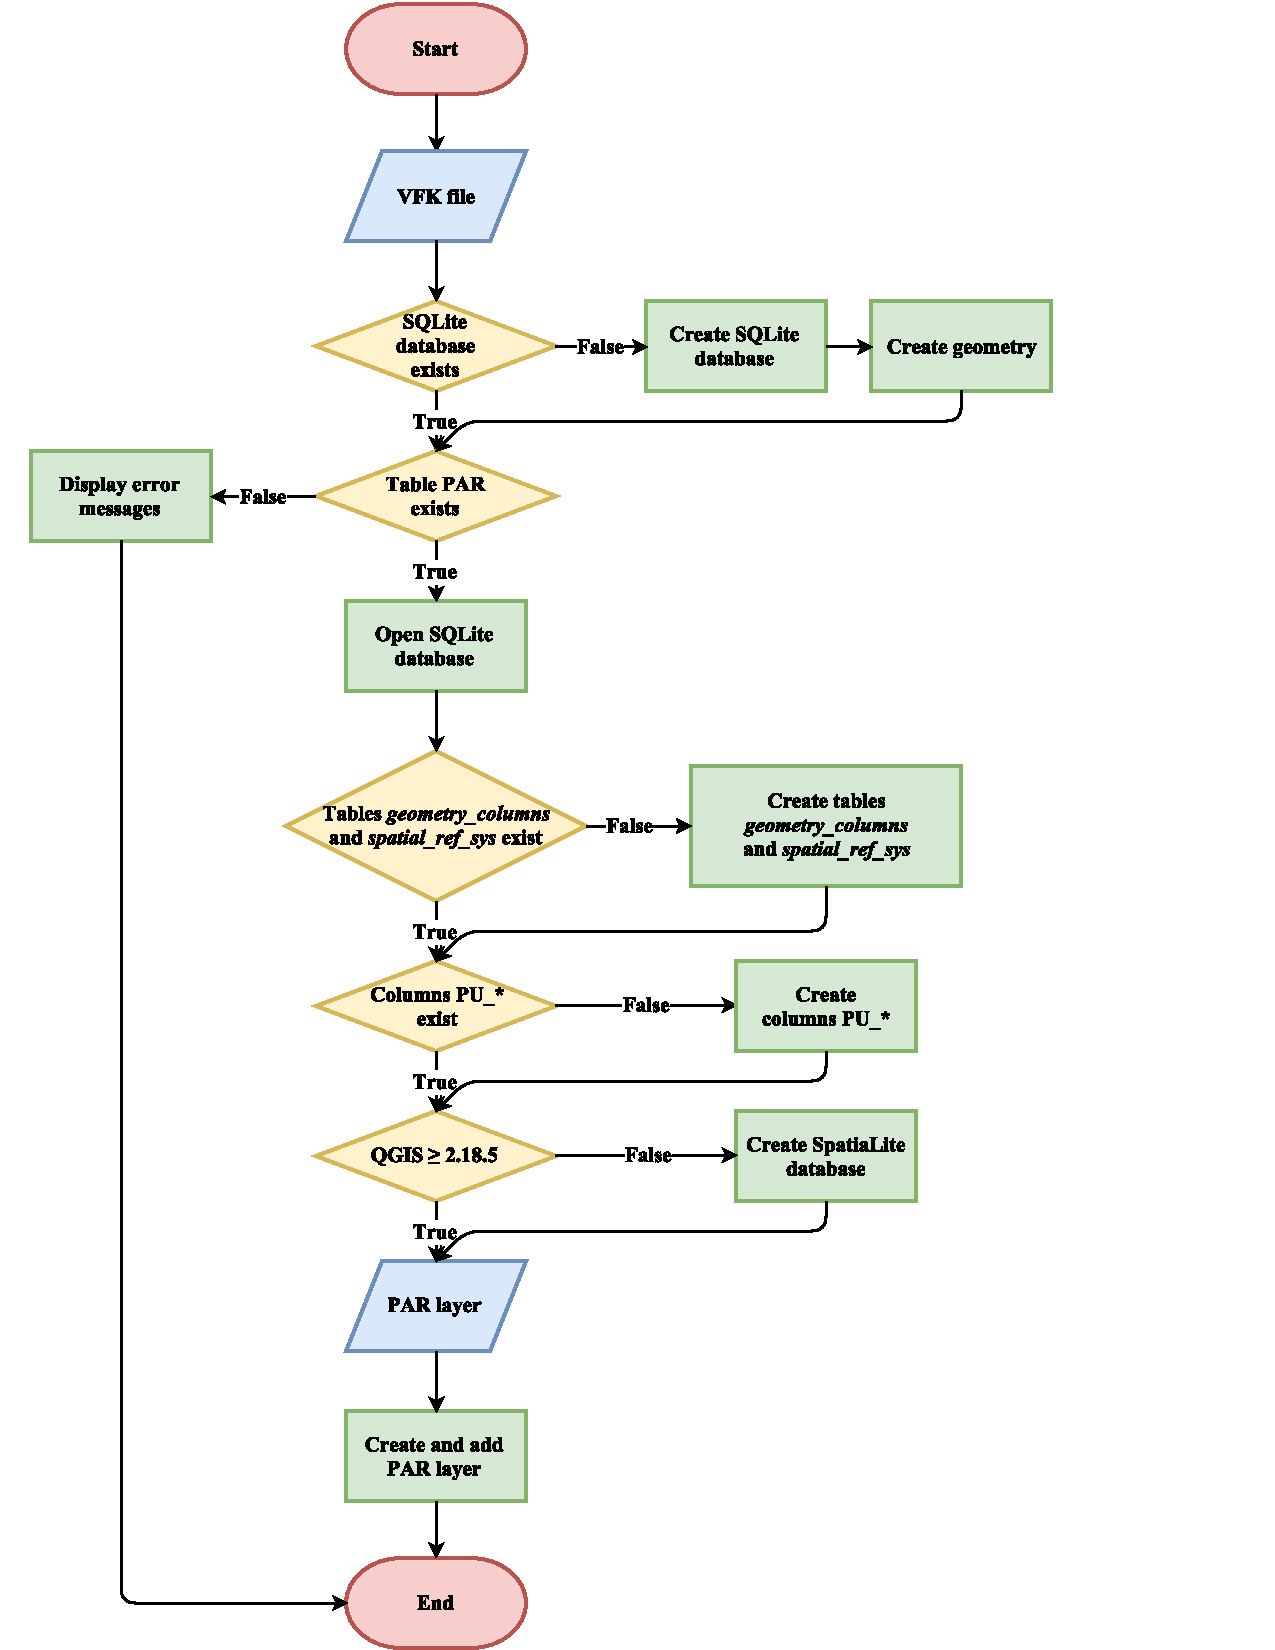
\includegraphics[width=1.2\textwidth]{./pictures/nacitani_vfk_souboru.pdf}
		\caption[Načtení \zk{VFK} souboru~– diagram
algoritmu]{Načtení \zk{VFK} souboru~– diagram algoritmu (zdroj: autor)}
		\label{fig:diagram_nacitani_vfk}
 	\end{figure}

\subsection{Symbologie vrstvy \texttt{\zk{PAR}}}
\label{symbologie_par}

Symbologie nahrané vrstvy parcel je dána podle předem připraveného QML
souboru, ve~kterém jsou definovány barvy podle druhů
pozemků. V~tabulce~\texttt{\zk{PAR}} je informace o~druhu pozemku
uvedena ve~sloupci \texttt{\detokenize{DRUPOZ_KOD}} (viz
tab.~\ref{tab:par_sloupce}), kódy druhů pozemku s~názvy se nachází v
tab.~\ref{tab:druhy_pozemku}.

\begin{table}[H]
    \begin{tabular}{|l|l|} \hline kód & název \\ \hline \hline
\texttt{2} & orná půda \\ \hline \texttt{3} & chmelnice \\ \hline
\texttt{4} & vinice \\ \hline \texttt{5} & zahrada \\ \hline
\texttt{6} & ovocný sad \\ \hline \texttt{7} & trvalý travní porost \\
\hline \texttt{10} & lesní pozemek \\ \hline \texttt{11} & vodní
plocha \\ \hline \texttt{13} & zastavěná plocha a nádvoří \\ \hline
\texttt{14} & ostatní plocha \\ \hline
    \end{tabular} \centering
    \caption[Druhy pozemků]{Druhy pozemků (zdroj
\citep{vyhlaska_357})}
    \label{tab:druhy_pozemku}
\end{table}

\newpage

\subsection{Atributová tabulka vrstvy \texttt{\zk{PAR}}}
\label{tabulka_par}

Tabulka parcel sama o~sobě obsahuje mnoho sloupců. Společně
se~sloupci, které přidává zásuvný modul, se stává nepřehlednou, proto
plugin všechny nepotřebné sloupce v~atributové tabulce skrývá. Kvůli
větší srozumitelnosti pro~uživatele navíc přidává sloupcům aliasy, viz
tab.~\ref{tab:viditelne_sloupce_aliasy_par}.

%%% ML: tabulka by mohla byt sirsi, potom by se text zbytecne nezalamoval
\begin{table}[H]
    \begin{tabular}{|l|l|} \hline název sloupce & alias \\ \hline
\hline \texttt{\detokenize{KMENOVE_CISLO_PAR}} & \texttt{KMENOVE
C. (PUV.)} \\ \hline \texttt{\detokenize{PU_PODDELENI_CISLA_PAR}} &
\texttt{PODDELENI C. (EDI.)} \\ \hline
\texttt{\detokenize{PODDELENI_CISLA_PAR}} & \texttt{PODDELENI
C. (PUV.)} \\ \hline \texttt{\detokenize{PU_KMENOVE_CISLO_PAR}} &
\texttt{KMENOVE C. (EDI.)} \\ \hline
\texttt{\detokenize{PU_KATEGORIE}} & \texttt{KATEGORIE} \\ \hline
\texttt{\detokenize{VYMERA_PARCELY}} & \texttt{VYMERA (SPI)} \\ \hline
\texttt{\detokenize{PU_VYMERA_PARCELY}} & \texttt{VYMERA (SGI)} \\
\hline
          \begin{tabular}{@{}l@{}}
\texttt{\detokenize{PU_VYMERA_PARCELY}} \\
\texttt{\detokenize{_ABS_ROZDIL}} \end{tabular} & \texttt{ROZ. VYMER}
\\ \hline
          \begin{tabular}{@{}l@{}}
\texttt{\detokenize{PU_VYMERA_PARCELY}} \\
\texttt{\detokenize{_MEZNI_ODCHYLKA}} \end{tabular} &
\texttt{MEZ. ODCH. ROZ. VYMER} \\ \hline
\texttt{\detokenize{PU_VZDALENOST}} & \texttt{VZDALENOST} \\ \hline
\texttt{\detokenize{PU_CENA}} & \texttt{CELK. CENA} \\ \hline
          \begin{tabular}{@{}l@{}} \texttt{\detokenize{PU_BPEJ}} \\
\texttt{\detokenize{_BPEJCENA_VYMERA_CENA}} \end{tabular}
& \begin{tabular}{@{}l@{}} \texttt{BPEJ KOD-CENA ZA M2} \\
\texttt{-VYMERA-CENA} \end{tabular} \\ \hline
\texttt{\detokenize{PU_MERITKO_PODKLADU}} & \texttt{MERITKO PODKL.} \\
\hline
    \end{tabular} \centering
    \caption[Vrstva \texttt{\zk{PAR}}~– viditelné sloupce
a~aliasy]{Vrstva \texttt{\zk{PAR}}~– viditelné sloupce a~aliasy (zdroj: autor)}
    \label{tab:viditelne_sloupce_aliasy_par}
\end{table}

\newpage

\section{Editace}
\label{editace}

Velmi důležitou činností během přípravné fáze pozemkových úprav je
určení obvodu pozemkové úpravy a~rozdělení parcel do~kategorií
(viz~\ref{obvod_a_predmet_pu}).

Algoritmus načtení \zk{VFK} souboru otvírá vrstvu parcel pomocí SQLite
Driveru\footnote{Ve~verzi programu QGIS nižší než~2.18.5 je vrstva
otevřená Spatialite Driverem, viz~\ref{nacteni_vfk_algoritmus}.},
takže ji lze editovat.

\subsection{Kategorie parcel}
\label{kategorie_parcel}

Kvůli zařazení parcel do~kategorií se během načítání přidává do~vrstvy
parcel sloupec \texttt{\detokenize{PU_KATEGORIE}} (alias
\texttt{KATEGORIE}), jehož datový typ je celé číslo
(\texttt{integer}). Zásuvný modul místo dlouhých názvů jednotlivých
kategorií používá číslice \texttt{0} - \texttt{2},
viz~tab~\ref{tab:kategorie_hodnoty}.

\begin{table}[H]
    \begin{tabular}{|l|l|} \hline hodnota & kategorie parcel \\ \hline
\hline \texttt{0} & mimo obvod \\ \hline \texttt{1} & v obvodu~–
neřešené \\ \hline \texttt{2} & v obvodu~– řešené \\ \hline
    \end{tabular} \centering
    \caption[Sloupec \texttt{PU\textunderscore KATEGORIE}~–
hodnoty]{Sloupec \texttt{PU\textunderscore KATEGORIE}~– hodnoty (zdroj: autor)}
    \label{tab:kategorie_hodnoty}
\end{table}

Plugin disponuje mechanismy pro~nastavení této hodnoty (viz ukázka
kódu~\ref{nastaveni_hodnoty_kategorie}) a~pro~výběr prvků v~kategorii
(viz ukázka kódu~\ref{vyber_v_kategorii}).

{\scriptsize
\begin{lstlisting}[style=python, caption={Kategorie parcel~– nastavení
hodnoty}, captionpos=b, label=nastaveni_hodnoty_kategorie,
backgroundcolor = \color{light-gray}, numbers=left]
fieldId = layer.fieldNameIndex('PU_KATEGORIE')

layer.startEditing() layer.updateFields()

for feature in features:
   if feature.attribute('PU_KATEGORIE') != value:
   id = feature.id()
layer.changeAttributeValue(id, fieldId, value)

layer.commitChanges()
\end{lstlisting}}

{\scriptsize
\begin{lstlisting}[style=python, caption={Kategorie parcel~– výběr
prvků v~kategorii}, captionpos=b, label=vyber_v_kategorii,
backgroundcolor = \color{light-gray}, numbers=left]
expression = QgsExpression("\"PU_KATEGORIE\" = {}".format(value))
features = layer.getFeatures(QgsFeatureRequest(expression))

ids = [feature.id() for feature in features]
layer.selectByIds(ids)
\end{lstlisting}}

\subsection{Vrstva obvodu}
\label{vrstva_obvodu}

Obvod pozemkové úpravy je území dotčené pozemkovými úpravami, patří
do~něj tedy parcely zařazené do~jednotlivých kategorií.

Bývá znázorňován tak, že všechny sousedící pozemky ve~stejné kategorii
tvoří pouze jeden prvek, u~kterého nejsou viditelné vnitřní
hranice. Tyto větší sloučené prvky je zvykem doplňovat o~popisky,
které značí, do~které kategorie náleží.

Zásuvný modul vytváří vrstvu obvodu na~základě sloupce
\texttt{\detokenize{PU_KATEGORIE}} ve~vrstvě parcel. Nejprve je
na~vrstvu \texttt{\zk{PAR}} zavolán nástroj \textit{Dissolve}
s~parametrem sloupce \texttt{\detokenize{PU_KATEGORIE}}. Díky tomu se
sousedící parcely v~jednotlivých kategoriích sloučí do~větších
celků. Program QGIS funguje tak, že prvky, které jsou tvořeny několika
body, liniemi, nebo polygony, mají pouze jeden popisek. Výstupem
nástroje \textit{Dissolve} mohou být i~multipolygony (prvky tvořeny
více polygony), proto je nutné zavolat funkci \textit{Multiparts
to~singleparts}, která problémové multipolygony rozdělí. Nakonec se
odstraní prvky, které mají nulovou hodnotu ve~sloupci
\texttt{\detokenize{PU_KATEGORIE}}, neboť takové prvky do vrstvy
obvodu nepatří. Ukázka kódu \ref{obvod_tvorba} obsahuje volání
nástrojů \textit{Dissolve} a~\textit{Multiparts to~singleparts}.

{\scriptsize
\begin{lstlisting}[style=python, caption={Vrstva obvodu~– tvorba},
captionpos=b, label=obvod_tvorba, backgroundcolor =
\color{light-gray}, numbers=left]
tempPerimeterLayerPath = processing.runalg('qgis:dissolve', layer,
                                           False, 'PU_KATEGORIE',
                                           None)['OUTPUT']
tempPerimeterLayer = QgsVectorLayer(tempPerimeterLayerPath,
                                    tempPerimeterLayerName, 'ogr')

processing.runalg('qgis:multiparttosingleparts', tempPerimeterLayer,
                  perimeterLayerFilePath)
perimeterLayer = QgsVectorLayer(perimeterLayerFilePath,
                                perimeterLayerName, 'ogr')
\end{lstlisting}}

\subsection{Symbologie vrstvy obvodu}
\label{symbologie_obvod}

Symbologie vrstvy obvodu se stejně jako u~vrstvy parcel řídí podle QML
souboru. V~popiscích vrstvy jsou hodnoty sloupce
\texttt{\detokenize{PU_KATEGORIE}}, jejich význam je popsán
v~tab.~\ref{tab:kategorie_hodnoty}. Popisky se zobrazují při jakémkoli
měřítku.

\subsection{Atributová tabulka vrstvy obvodu}
\label{tabulka_obvod}

Vrstva obvodu se vytváří z~vrstvy parcel, ovšem pouze informace
o~kategorii je pro~obvod relevantní. Z~toho důvodu je viditelný pouze
sloupec \texttt{\detokenize{PU_KATEGORIE}}, viz
tab.~\ref{tab:viditelne_sloupce_aliasy_obvod}.

\begin{table}[H]
    \begin{tabular}{|l|l|} \hline název sloupce & alias \\ \hline
\hline \texttt{\detokenize{PU_KATEGORIE}} & \texttt{KATEGORIE} \\
\hline
    \end{tabular} \centering
    \caption[Vrstva obvodu~– viditelné sloupce a~aliasy]{Vrstva
obvodu~– viditelné sloupce a~aliasy (zdroj: autor)}
    \label{tab:viditelne_sloupce_aliasy_obvod}
\end{table}

%%% ML: je nutne aby podkapitola zacinala vzdy na nove strance?, pokud
%%% to tak mas jinde v textu tak to nech
\newpage

\section{Kontroly a analýzy}
\label{kontroly_analyzy}

Během přípravné fáze je nutné zkontrolovat soulad \zk{SPI} a~\zk{SGI}
dat katastru nemovitostí, ověřit správnost rozdělení parcel~do
kategorií a~také provést analýzy pro~sestavení vstupních soupisů
nároků vlastníků.

\subsection{Kontroly}
\label{kontroly}

\subsubsection{Kontrola - obvodem}
\label{kontrola_obvodem}

Kontrola \textit{obvodem} slouží k~výběru parcel, které se nenachází
kompletně uvnitř vrstvy obvodu.

%%% ML: z textu neni uplne zrejme, ze jde o nastroje QGISu, alespon
%%% zde jsem to explicitne uvedl
Do~algoritmu vstupuje vrstva parcel a~vrstva obvodu. Použit je nástroj
systému QGIS \textit{Select by~location} s~geometrickým predikátem
\textit{within} a~poté je zavolána funkce pro~převrácení výběru prvků,
viz ukázka kódu~\ref{kontrola_obvodem_kod}.

{\scriptsize
\begin{lstlisting}[style=python, caption={Kontrola \textit{obvodem}~–
výběr prvků}, captionpos=b, label=kontrola_obvodem_kod,
backgroundcolor = \color{light-gray}, numbers=left]
processing.runalg('qgis:selectbylocation', layer, perimeterLayer,
                  u'within', 0, 0)

layer.invertSelection()
\end{lstlisting}}

\subsubsection{Kontrola - není v SPI}
\label{kontrola_neni_v_spi}

Jak vyplývá z~názvu, kontrola \textit{není v~SPI} provádí výběr
parcel, které nejsou uvedeny v~souboru popisných informací. Pro výběr
používá sloupec \texttt{\detokenize{KMENOVE_CISLO_PAR}}, neboť patří
mezi povinně vyplněné \citep{struktura_vfk}. Pokud má parcela tento
sloupec prázdný, znamená to, že se jedná o~chybu nebo nově vytvořenou
parcelu.

{\scriptsize
\begin{lstlisting}[style=python, caption={Kontrola \textit{není
v~SPI}~– vzorec pro~výběr prvků}, captionpos=b,
label=kontrola_spi_kod, backgroundcolor = \color{light-gray},
numbers=left]
expression = QgsExpression("\"KMENOVE_CISLO_PAR\" is null")
\end{lstlisting}}

\subsubsection{Kontrola - není v mapě}
\label{kontrola_neni_v_mape}

Výsledkem kontroly \textit{není v~mapě} je výběr parcel, které mají
prázdnou geometrii a~tudíž se nezobrazují v~mapovém okně. Vybrány jsou
%%% ML: co presne znamena nevalidni geometrie (kratce uvest)
též parcely s~nevalidní geo\-metrií.

{\scriptsize
\begin{lstlisting}[style=python, caption={Kontrola \textit{není
v~mapě}~– vzorec pro~výběr prvků}, captionpos=b,
label=kontrola_mapa_kod, backgroundcolor = \color{light-gray},
numbers=left]
expression = QgsExpression("$geometry is null")
\end{lstlisting}}

\subsubsection{Kontrola - výměra nad mezní odchylkou}
\label{kontrola_vymera}

Kontrola \textit{výměra nad~mezní odchylkou} zjišťuje, jestli~rozdíl
mezi výměrou dle~souboru popisných informací a~výměrou danou souborem
geodetickým informací překračuje mezní odchylku. Hodnota mezní
odchylky závisí na~kódu kvality nejméně přesně určeného lomového bodu
na~hranici parcely \citep{vyhlaska_357}, viz
tab.~\ref{tab:odchylky_vymer}. Pro~digitalizované parcely se kód
kvality podrobných bodů určí podle~měřítka podkladové mapy, viz
tab.~\ref{tab:kody_kvality_digit}.

Algoritmus z~vrstvy parcel nejdříve vyfiltruje prvky, které mají
validní geometrii a~zadanou výměru podle \zk{SPI}. Poté v~cyklu všemi
takovými prvky prochází. Pro~identifikaci parcel, které byly
digitalizované, slouží sloupec
\texttt{\detokenize{PU_MERITKO_PODKLADU}}. Hodnota \texttt{1} značí,
že parcela nemá validní geometrii, jiné číslo udává měřítko podkladové
mapy. Pokud je tedy v~tomto sloupci uvedeno číslo různé od~\texttt{1},
znamená to, že~se jedná o~digitalizovanou parcelu. V~takovém případě
algoritmus zjistí kód kvality podrobných bodů podle
%%% ML: co presne znaci nejvetsi kod kvality?
tab.~\ref{tab:kody_kvality_digit}. Pomocí lomového bodu s~největším
kódem kvality se vypočte mezní odchylka výměr a~porovná se
s~absolutním rozdílem výměr dle~\zk{SPI} a~\zk{SGI}. Když je mezní
odchylka překročena, přidá se parcela do~výběru. V~momentě, kdy už není
k~dispozici žádný další prvek, se kontrola ukončí. Celý postup
znázorňuje diagram na obr.~\ref{fig:diagram_vymera}.

\subsubsection{Kontrola - bez vlastníka}
\label{kontrola_bez_vlastnika}

Kontrola \textit{bez~vlastníka} používá sloupec
\texttt{\detokenize{TEL_ID}} pro~výběr parcel, které jsou
bez~vlastníka, tzn. že~nemají přiřazený list vlastnictví, viz ukázka
kódu~\ref{kontrola_vlastnik_kod}. Takové parcely se označují jako
\textit{LV~0}.

{\scriptsize
\begin{lstlisting}[style=python, caption={Kontrola
\textit{bez~vlastníka}~– vzorec pro~výběr prvků}, captionpos=b,
label=kontrola_vlastnik_kod, backgroundcolor = \color{light-gray},
numbers=left]
expression = QgsExpression("\"TEL_ID\" is null")
\end{lstlisting}}

	\begin{figure}[H] \centering
		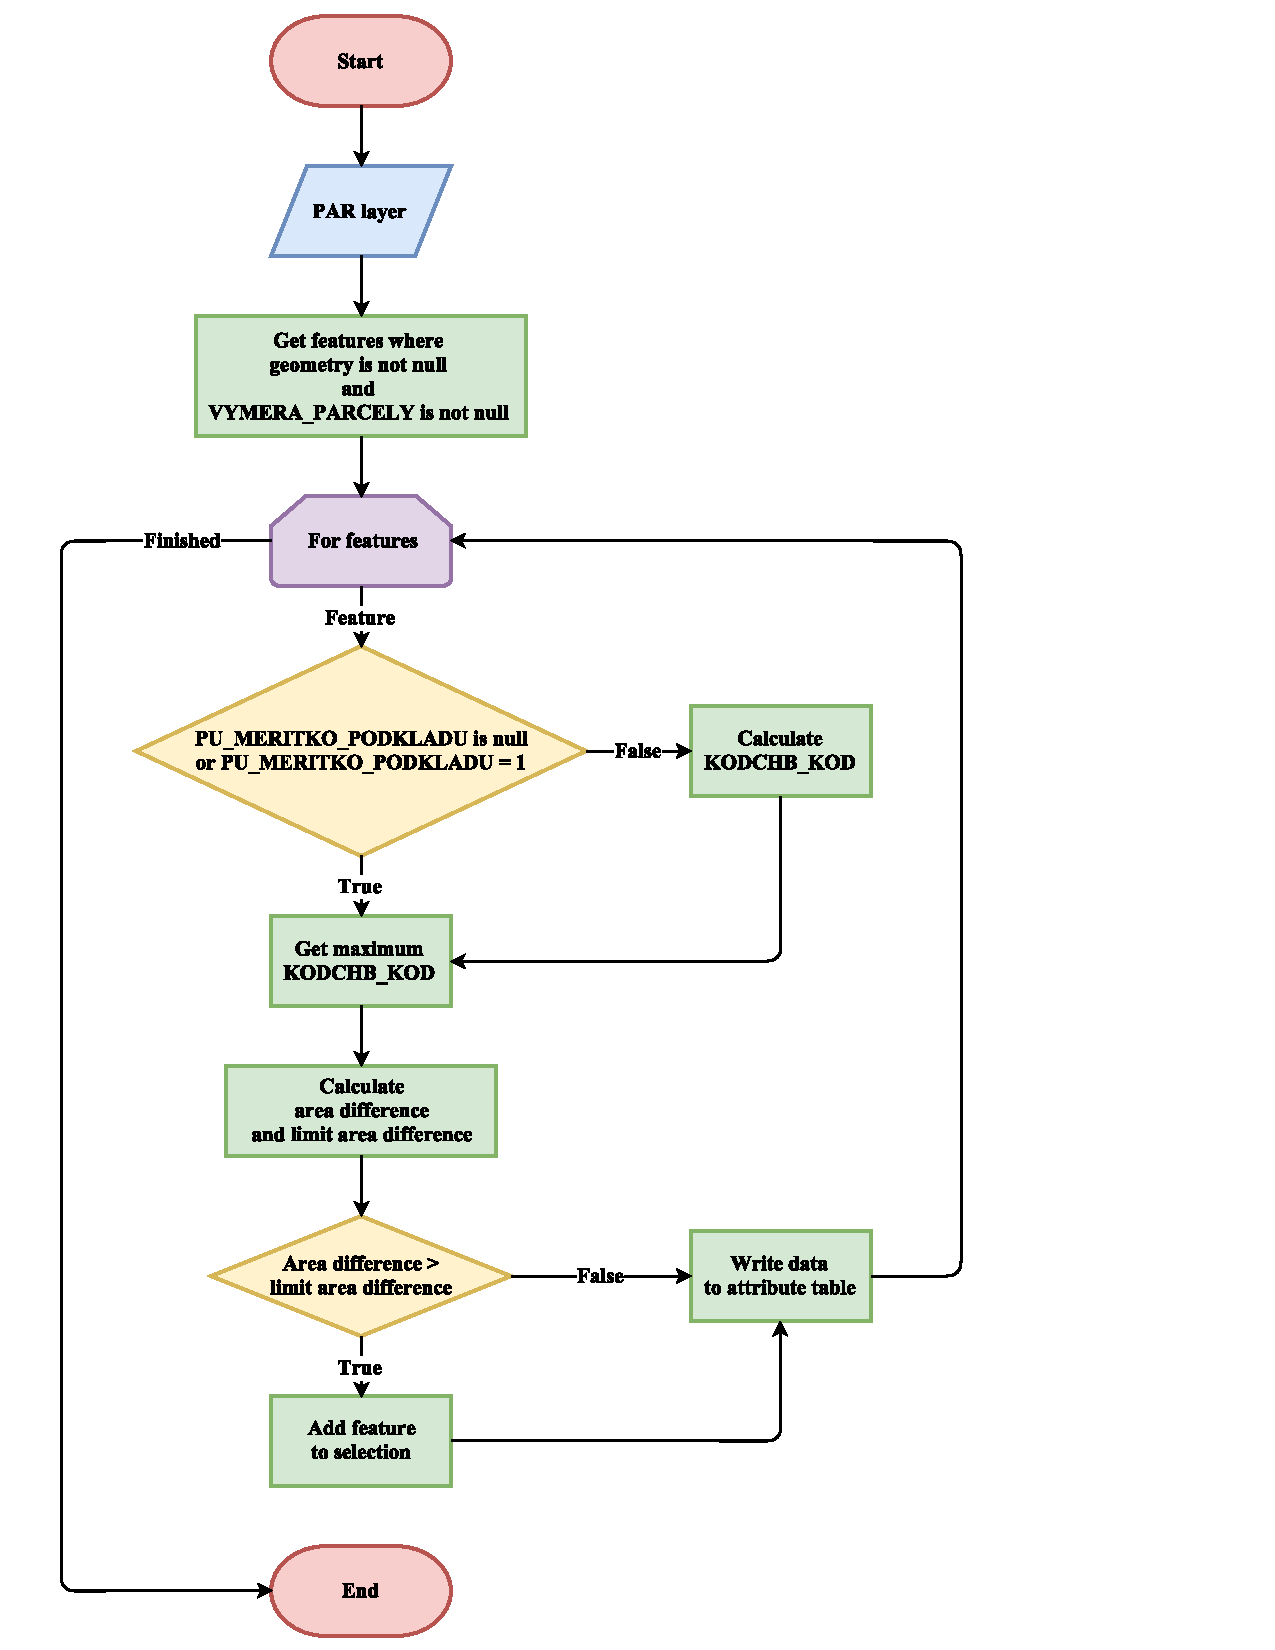
\includegraphics[width=1.2\textwidth]{./pictures/vymera.pdf}
		\caption[Kontrola \textit{výměra nad mezní
odchylkou}~– diagram algoritmu]{Kontrola \textit{výměra nad mezní
odchylkou}~– diagram algoritmu (zdroj: autor)}
		\label{fig:diagram_vymera}
 	\end{figure}

\subsection{Analýzy}
\label{analyzy}

\subsubsection{Analýza - měření vzdálenosti}
\label{analyza_vzdalenosti}

Analýza \textit{měření vzdálenosti} určuje pro~všechny parcely
v~kategorii \textit{v~obvodu~- řešené (2)} vzdálenost jejich těžiště
od~referenčního bodu, viz ukázka
kódu~\ref{analyza_vzdalenost_vypocet_vzdalenosti_teziste_od_ref_bodu}. Výsledné
zaokrouhlené hodnoty v~metrech ukládá do~sloupce
\texttt{\detokenize{PU_VZDALENOST}}

Do~kontroly kromě vrstvy parcel vstupuje i~vrstva referenčního bodu,
která musí obsahovat právě jeden prvek a~kvůli zamezení neočekávaných
výsledků musí mít stejný souřadnicový systém jako vrstva parcel.

{\scriptsize
\begin{lstlisting}[style=python, caption={Analýza \textit{měření
vzdálenosti}~– výpočet vzdálenosti těžiště\newline od~referenčního
bodu}, captionpos=b,
label=analyza_vzdalenost_vypocet_vzdalenosti_teziste_od_ref_bodu,
backgroundcolor = \color{light-gray}, numbers=left]
centroid = geometry.centroid().asPoint()
distanceDouble = sqrt(refPoint.sqrDist(centroid))
distance = int(round(distanceDouble))
\end{lstlisting}}

\subsubsection{Analýza - oceňování podle BPEJ}
\label{analyza_bpej}

Analýza \textit{oceňování podle BPEJ} vypočítá cenu pozemku na~základě
vrstvy hranic \zk{BPEJ}.

Pro~určení ceny za~metr čtvereční jednotlivých kódů \zk{BPEJ} analýza
používá číselník \zk{BPEJ} z~Českého úřadu zeměměřičského a
katastrálního\footnote{Informace o~číselníku jsou dostupné
na~\url{https://goo.gl/uXf8FC}. Samotný číselník lze stáhnout
z~\url{http://www.cuzk.cz/CUZK/media/CiselnikyISKN/SC_BPEJ/SC_BPEJ.zip?ext=.zip}.}. Tento
číselník je aktualizován každý den kolem třetí hodiny ranní.

Do~algoritmu vstupují vrstvy \texttt{\zk{PAR}} a~hranice \zk{BPEJ},
na~které je volán nástroj systému QGIS vektorového překryvu \textit{Union}. Poté se
zkontroluje aktuálnost číselníku \zk{BPEJ}. Jestliže číselník není
aktuální a~lze se připojit k~internetu\footnote{Pro testování
internetového připojení byla zvolena adresa
%%% ML: je potreba testovat pripojeni zvlast? Nestacilo by se pokusit
%%% stahnout ciselnik a pripadne o tom informovat uzivatele? Ted to
%%% tak ale uz nech.
\url{https://www.google.com}.}, stáhne zásuvný modul nový
číselník. V~dalším kroku se z~nejnovějšího dostupného číselníku
přečtou data a~vypočítá se cena. Do~atributové tabulky se zapíše nejen
cena celková (sloupec \texttt{\detokenize{PU_CENA}}), ale~také cena
za~metr čtvereční, výměra a~cena dle jednotlivých bonit v~příslušné
parcele (sloupec
\texttt{\detokenize{PU_BPEJ_BPEJCENA_VYMERA_CENA}}). Může se stát, že
uživatel zvolí špatný sloupec, nebo že kód \zk{BPEJ} nebude uveden
v~číselníku. V~takovém případě plugin vybere ve~vrstvě obvodu prvky,
pro~které nenalezl ceny, a~informuje uživatele o~problému.

Algoritmus počítá i~s~možností změny adresy pro~stažení číselníku,
když tato situace nastane, oznámí to uživateli.

Princip algoritmu je znázorněn na obr.~\ref{fig:diagram_bpej}.

	\begin{figure}[H] %%\centering
		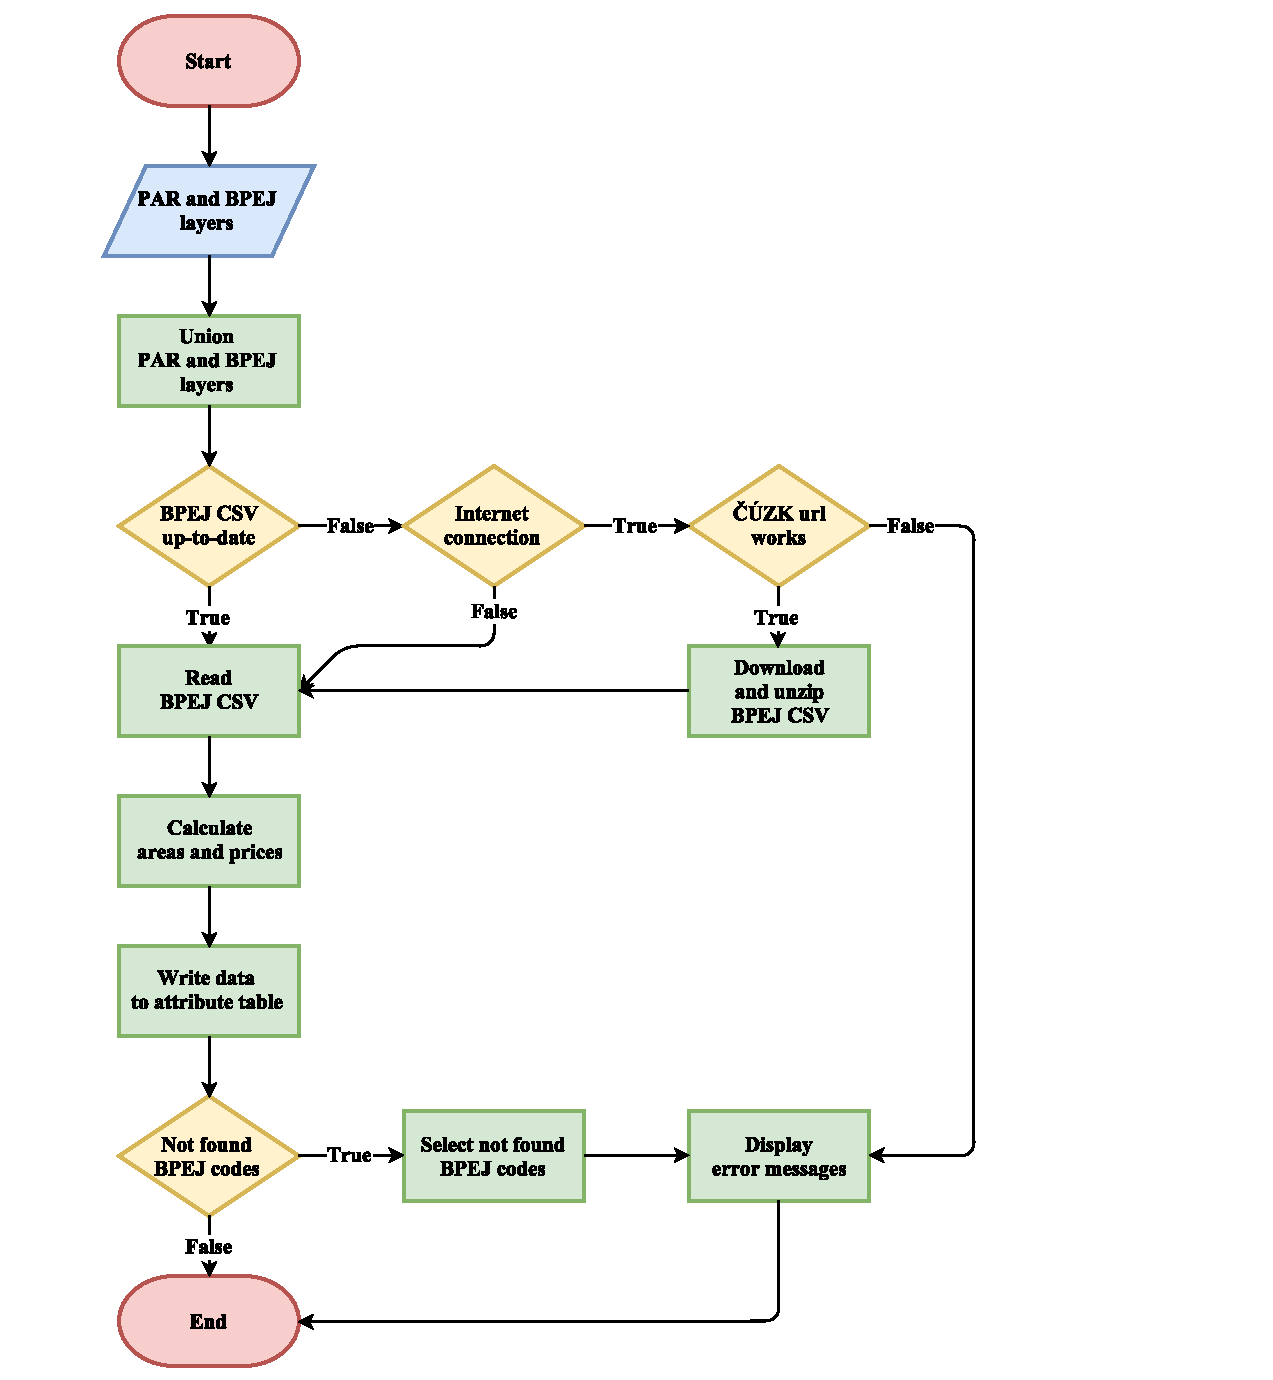
\includegraphics[width=1.2\textwidth]{./pictures/bpej.pdf}
		\caption[Analýza \textit{oceňování podle BPEJ}~–
diagram algoritmu]{Analýza \textit{oceňování podle BPEJ}~– diagram
algoritmu (zdroj: autor)}
		\label{fig:diagram_bpej}
 	\end{figure}
